%
% Paper to be submitted to the 2013 IEEE International Conference
% on Technologies for Homeland Security (HST'13), Boston,
% Massachusetts, 12--14 November 2013.
%
% For information on this file please contact Joe Loughry at
% Tel. +1 303 221 4380 (time zone GMT minus 7 hours) or Email:
% joe.loughry@stx.ox.ac.uk
%

\documentclass[10pt,letterpaper,conference]{IEEEtran}

% sort and compress citation numbers in IEEE style:
\usepackage{cite}

\usepackage[english,british]{babel}
% \usepackage[pdftex]{graphicx}
\usepackage{graphicx}

\usepackage[cmex10]{amsmath}
\interdisplaylinepenalty=2500

\usepackage{array}
% Frank Mittelbach's and David Carlisle's array.sty patches and improves
% the standard LaTeX2e array and tabular environments to provide better
% appearance and additional user controls. As the default LaTeX2e table
% generation code is lacking to the point of almost being broken with
% respect to the quality of the end results, all users are strongly
% advised to use an enhanced (at the very least that provided by array.sty)
% set of table tools. array.sty is already installed on most systems. The
% latest version and documentation can be obtained at:
% http://www.ctan.org/tex-archive/macros/latex/required/tools/

\usepackage{caption}
\usepackage[caption=false,font=footnotesize]{subfig}

\usepackage{fixltx2e}

\usepackage{comment}

\usepackage{url}

% *** Do not adjust lengths that control margins, column widths, etc. ***
% *** Do not use packages that alter fonts (such as pslatex).         ***
% There should be no need to do such things with IEEEtran.cls V1.6 and later.
% (Unless specifically asked to do so by the journal or conference you plan
% to submit to, of course. )

% correct bad hyphenation here
\hyphenation{op-tical net-works semi-conduc-tor}

\begin{document}

\title{A Model of Certifier and Accreditor Risk Calculation for Multi-Level Systems}

\author{
	\IEEEauthorblockN{Joe Loughry}
	\IEEEauthorblockA{Doctoral Student in the Department of Computer Science \\
		University of Oxford \\
		Wolfson Building, Parks Road \\
		Oxford, OX1 3QD, UK \\
		Email: joe.loughry@stx.ox.ac.uk \\
		Tel: +1 303 221 4380
	}
}

\maketitle

\begin{abstract}
	From direct observation of the certification (post--software-development) and accreditation
(pre-installation) testing of cross domain systems used for the interconnection of classified
security domains in U.S.\ and U.K.\ defence and intelligence community systems, certain
characteristic behavioural patterns have been noted.  The savvy developer
can use these to exert a measure of control over the duration and cost of certification testing
and to predict the likely direction and magnitude of the residual risk calculation performed
by security accreditors in multi-lateral, multi-level, collateral, and compartmented site
accreditations.  DCID 6/3, Common Criteria, DIACAP, and ICD 503 testing efforts across the
evolution of a long-lived cross domain software development programme were examined using
grounded theory methodology.  Whilst discovered through investigation of classified cross
domain system testing inefficiencies, it is believed that the principles are applicable more
widely to privacy-sensitive areas such as electronic health care, financial, and law enforcement
record keeping systems.  The first thing found was a syndrome of pathological regressive
interactions amongst software developers, managers, independent verification and validation
contractors, penetration testers, and certification authorities that resulted in schedule
slippage during the certification testing phase and, in the accreditation phase, ineffective
duplication of testing with no corresponding improvement in residual risk.  To understand why
these problems occurred, an abstract model of how security accreditors agree upon the true
level of residual risk in multi-level cross domain system installations was developed.  The
model is powerful enough to handle collateral, SCI, and international cross domain systems
with any number of endpoints.  It works by establishing the visibility of threats,
vulnerabilities, and mitigations from each data owner's perspective according to the
associated accreditor's clearance over the space of all possible multi-level configurations,
then identifying the smallest set of covert-channel--like information flows necessary to
reach a concord about residual risk without violating the global security policy.  Conventional
wisdom holds that security rules should be strictly enforced, but it is shown that under present
regulations, some desirable information flows are inhibited and other undesirable information
flows are forced.  Paradoxically, it is sometimes the case that relaxing the rules actually
improves security.


\end{abstract}

\def\IEEEkeywordsname{Index Terms}

% update this with valid keywords from http://www.computer.org/mc/keywords/keywords.htm

\begin{IEEEkeywords}
	cross domain system, certification and accreditation,
	security test and evaluation, certification test and evaluation.
\end{IEEEkeywords}

\IEEEpeerreviewmaketitle

\section{Introduction}

It is generally believed that
certification and accreditation testing of cross domain systems takes more time than it ought
to and costs far more than necessary. Some of the reasons for this frustrating mis-allocation
of resources lie in the observable duplication of effort that seems to be characteristic of
cross domain solution security certification testing and cross domain system accreditation, as
fully described in previous work \cite{Loughry2010a,Loughry2012a}. This paper describes progress
toward a theory of cross domain security certification and accreditation deriving from long-term
observation of a portion of the evolution of a representative cross domain solution for which
software development began in 1992. Through more than twenty years of continuous maintenance and
enhancement since, the software underwent numerous security evaluations by agencies with different
testing criteria, aims, methods, and outcomes. Not all the outcomes were successful. It is
believed that the contrast between successful and unsuccessful security testing activities of a
succession of versions of the same software through multiple generations of security testing
criteria offers a chance to find underlying principles that are more difficult to discern in the
typical instance of short-run product cycles that are otherwise characteristic of the cross
domain software development ecosystem.

\subsection{Certification and Accreditation of Cross Domain Systems}

Cross domain systems are the backbone of interconnected networks of classified information
processing systems. While not formally limited to classified information---the same principles
apply to any multi-level security problem, for example the separation of engineering design
information from marketing and accounting departments in a company, of financial trading and
demand deposit functions in a merchant bank, chain of custody of evidence in law enforcement
applications, or the accumulation, protection, and use of privacy-sensitive
electronic health care records---this research, however, was done on the developers, installers,
testers, and users of a cross domain solution designed for handling classified information in
military and intelligence community environments.

Cross domain systems are what get installed in the field; they are built from components that
include cross domain solutions. A cross domain solution is really a type of router, but often
with additional capabilities at the Application layer atop the OSI model that go beyond `deep
packet inspection' to include, sometimes, data format transliteration, content-aware message
switching, and automatic sanitisation. Cross domain solutions are sometimes called `guards'.

\subsubsection{Certification}

Testing of cross domain solutions and cross domain systems is done in two phases independent of
the developer's own regression and functional tests. Every new or significantly updated version
of cross domain solution software must undergo certification testing and approval for use
by the responsible government agency before it can be approved for use in handling classified
information. Certification testing is usually performed by both Independent Verification and
Validation (IV\&V) contractors---who perform functional tests to verify that the product
does everything it is supposed to do and nothing it is not supposed to do---and by
penetration testers---commonly specialists employed by government agencies---who do more exotic
and open-ended tests, searching for undiscovered vulnerabilities.

\subsubsection{Accreditation}

Once a cross domain solution has passed certification testing at the end of the development
phase, it is approved for use in assembling cross domain systems, which are the things actually
connected to customer networks. No cross
domain system can be approved to operate and connect to classified information, however, before
it has passed accreditation testing. Accreditation is the process of testing and approving
a particular cross domain system, consisting of a particular cross domain solution connected to
particular networks in a particular place, processing particular types of information, for a
limited amount of time. Accreditation testing focusses on the details of
particular data formats, transformations, rules, and communicating end-points. Because
accreditation testing is done to the satisfaction of the accreditor---a government official whose
job it is to accept personal responsibility for the correct operation of the cross domain system in
production, and who is not the same person as the certification authority---accreditation testing
is often seen to duplicate functional testing performed during the certification phase as well as,
to some extent, specialised penetration testing that can be performed in the different and specific
environment of the installation site.

\subsection{Problems with Certification and Accreditation}

It might be argued that the present level of security of these systems is adequate, and therefore
we know a reasonable upper bound on cost and time of security testing, but it may also be
argued either that the level of security assurance is too high---impacting ship sailing schedules
in the Navy---or too low, as in the Manning and Snowden cases,
both of which \emph{might} have been stopped by a cross domain guard
\cite[Chapter 1]{Loughry2012b}. In addition, it is arguable that onerous certification and
accreditation requirements discourage the introduction of innovative technologies to the problem,
miring users in out-dated, under-functioning systems for lack of alternatives.

What is known without doubt is that certification and accreditation testing of cross domain
solutions and systems is duplicative of effort; this is observable. What was not understood until
recently, however, is the interactions between people during the process that yield insight into
their informal and formal communication channels. This research aims to understand the
reasons for security testing inefficiency with the goal of eliminating unnecessary redundancies in
the process.

\section{Methodology}\label{section:methodology}

The author was a participant observer in the software development and certification and
accreditation testing of a leading cross domain solution product, from 1998--2012. During this
time the software, here referred to as `$R$', underwent certification testing at least seven
times under three different
criteria---DCID 6/3, Common Criteria (CC), and ICD 503---in addition to hundreds of accreditations.
For three intervals in approximately 1999, 2004--6, and 2010--11, access to project records was
obtained for
research purposes. These encompass one abortive, one failed, and one completely successful security
certification and accreditation effort of a single product.

Because the same group of people were largely engaged in developing and testing the software,
through a series of versions, during all three of these times, it is believed that the
methodology used here provides a measure of control over confounding factors. Controlled
experiments are often unfeasible in software engineering due to the high cost of projects
\cite{McCue1978,Rost2011}. For this reason, a grounded theory approach was used instead
\cite{Glaser1967}.
Grounded theory methodology is suitable to the form of the data available from the three projects,
in which the author was a participant on the former projects and a non-participant observer on the
latter; in exchange for access to telephone conference calls over the lifetime of the third project,
the author minuted meetings between the developer and certifiers and accreditors and wrote some
technical reports for the developer.

\subsection{Participant Observation}

In 1999 the author assisted with the preparation of `evaluatable evidence', of the type that would
be used for a CC security evaluation, for the $R_0$ system. The intent was never to submit the
evidence for validation or certification, but a Security Target (ST) was written describing
the Security Functional Requirements to be claimed, and existing design documentation and software
development process and life-cycle documentation collected in support of the Security Assurance
Requirements specified at the Evaluation Assurance Level desired, comprising the evidence package.

Several years later, a foreign customer requested CC certification of the $R'$ version of the
software. The old evidence package was examined and found to be unusable because $R'$ had new
features that were not in $R_0$, and besides lacked some functionality of $R$ for export control
reasons. The author began writing a new ST for $R'$ and the latest process and life-cycle
documentation was added to the evidence package. It was not so easy to locate up-to-date design
documentation, however; the government sponsor of $R$ had, in the intervening years, refused to
pay for updating the design documents and these had fallen out of date. Problems were encountered
by the developer as a result during the validation phase. For reasons unrelated to $R'$, the
customer unexpectedly cancelled the project shortly before the evaluation phase was scheduled to
begin. CC certification was never achieved, although it should be emphasised that $R$ did not
fail security testing. The security evaluation effort, at a cost of approximately \$1.5 million,
failed to achieve its objective.

\begin{figure*}[!t]
    \centering
	% 'trim' specifies how much to remove from left, bottom, right, and top
	% edges of an A4 size PDF page.
	% \includegraphics[width=\textwidth,trim=24mm 129mm 24mm 46mm, clip]{network_grounded_theory_improved_layout_Type_1_fonts_embedded.pdf}
	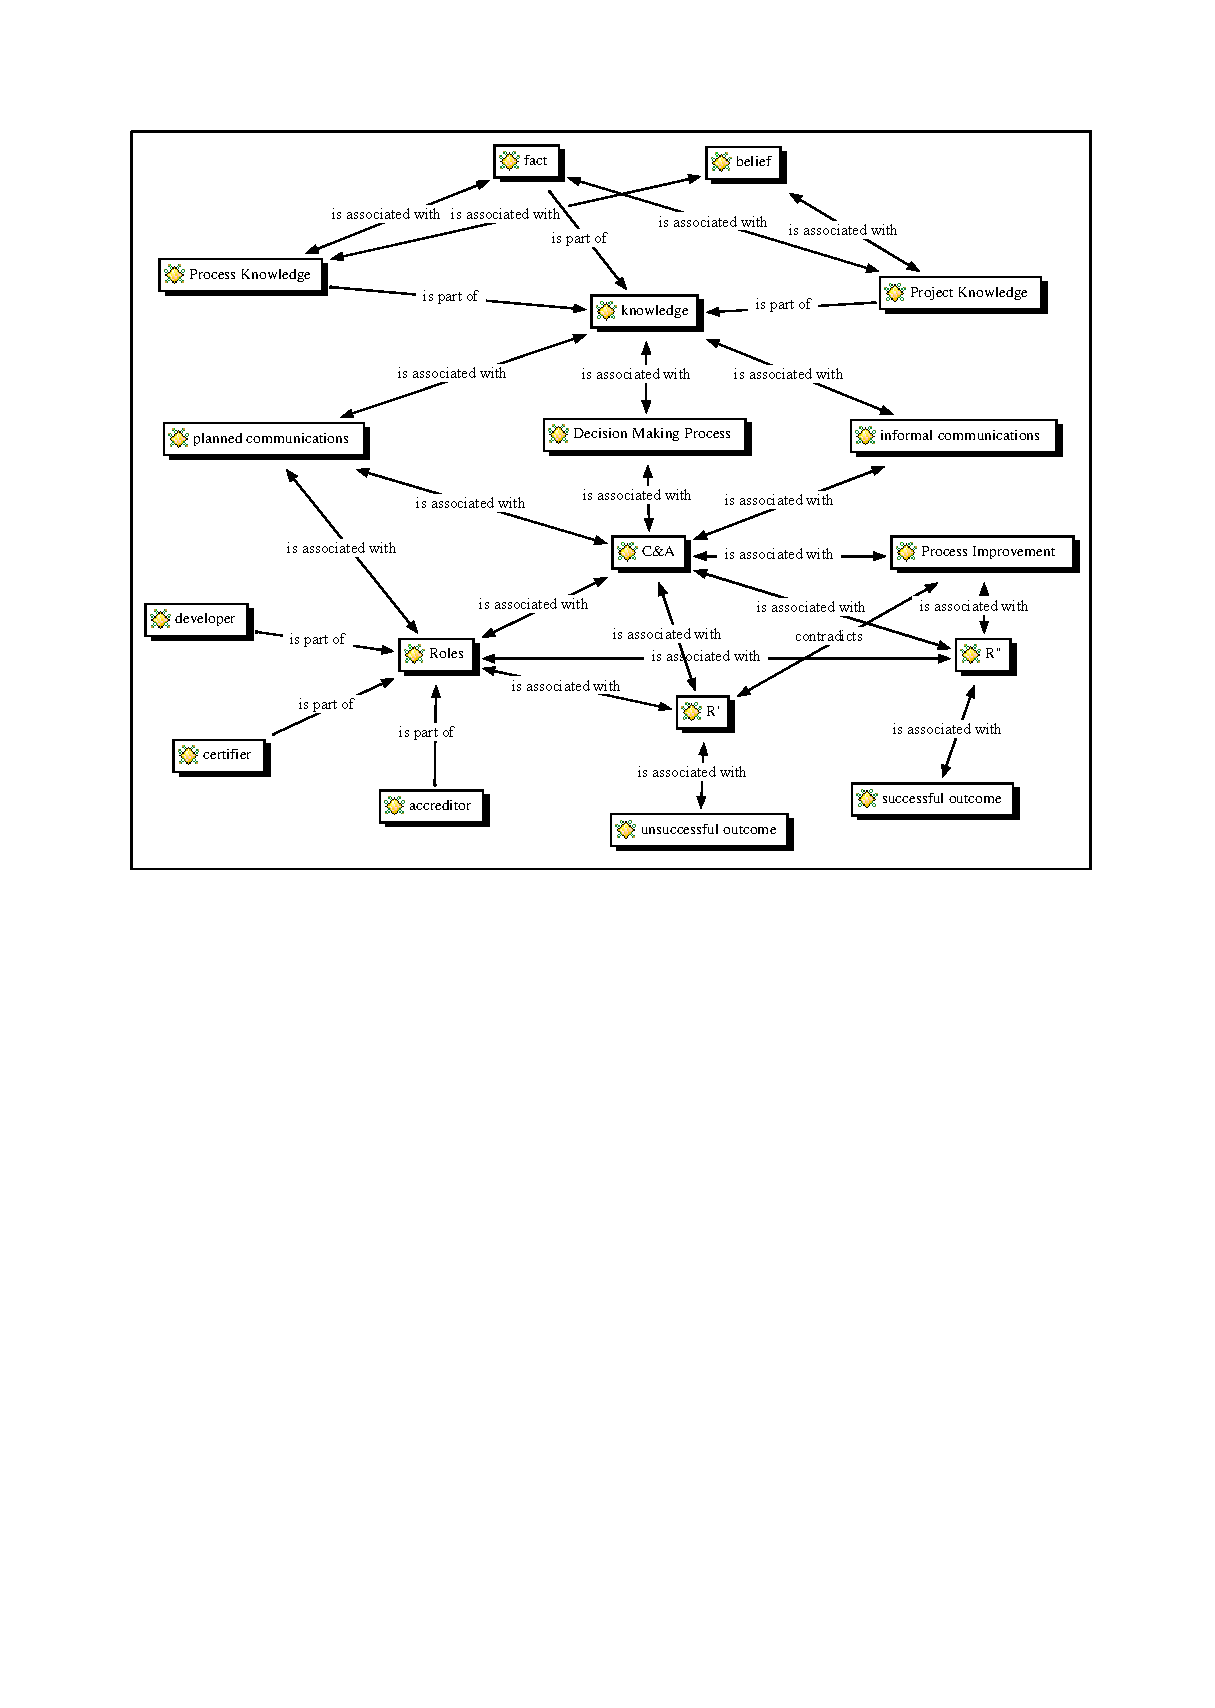
\includegraphics[width=\textwidth,bb=68 409 532 766]{network_grounded_theory_scaled_100.eps}
	\caption{Grounded theory found in the $R_0$, $R'$, and $R''$
		certification and accreditation case studies (adapted from \cite[Ch.\ 5]{Loughry2012b}).}
	\label{figure:grounded-theory}
\end{figure*}

\subsection{Non-Participant Observation}

The third set of project records was obtained for study in 2010--12 during the certification
testing of $R''$, a major version update to $R$. Particularly interesting about the effort this
time was it was the first cross domain certification and accreditation done under a new set of
testing criteria, ICD 503, which replaced DCID 6/3. None of the developer, certification authority,
testers, or accreditors were familiar with the security controls (from NIST SP 800-53) and risk
management framework (NIST SP 800-37) to be used. The author took minutes of numerous telephone
conference calls involving the developer, certification authority, IV\&V contractors, penetration
testers, regression testers, and accreditors from the beginning of the $R''$ certification through
the end of the first accreditation of a cross domain system incorporating $R''$. The certification
and accreditation of $R''$ were completely successful.

\section{Results}

The grounded theory model derived from the data collected in Section~\ref{section:methodology}
is shown in \figurename~\ref{figure:grounded-theory} and presented fully in reference
\cite{Loughry2012b}. However, a brief overview of some of the more interesting results is
possible here.

A strongly suggestive association was found between the occurrence of informal communications
during certification testing activities and successful outcomes. Specifically, precursor
communications carrying news of the results of regression testing and penetration testing in $R''$
often preceded planned formal communications, i.e., reports, by an interval sufficiently long to be
helpful in immediate-term scheduling. Precursor communications were not seen in $R'$, although
informal follow-on communications were. Furthermore, the $R''$ case study showed
examples of informal process improvement communication that were completely absent in $R'$.

Information asymmetry appeared to play a role in developer--certifier relations throughout the
$R''$ certification, extending into the accreditation phase. Penetration testers, especially in a
classified environment, as this was, are caught in a dilemma; they can inadvertently teach the
developer to avoid poor practices at the cost of `using up' some of the penetration testers'
proprietary vulnerability-finding techniques every time. This comes at a cost to the penetration
testers, who must then replenish their store of new tricks through independent research. Obviously
the goal of penetration testers in certification and accreditation testing is to harden the device
under test, but this knowledge asymmetry between developer and tester evidently drives some of the
personality conflicts observed in the $R''$ data. Knowledge is continually transferred in multiple
directions and not only through formal channels. In fact, belief appears to be qualitatively as
influential as fact in the continuous updating of process knowledge and project knowledge that
drive the decision making process controlling certification and accreditation.

\section{Interpretation}

It was just this sort of imbalance, as seen between the government security penetration testers
and the developer during the certification phase that suggested the following approach
applicable to the accreditation phase. What emerged was an abstract model of accreditor behaviour
sufficient to describe all possible configurations of accreditors that have been seen in the field.
Accreditors represent data owners and their associated systems that connect to a cross domain
system. Accreditors perform a risk assessment decision based on their perceived value of `their'
information, their perceived effectiveness of the security controls implemented by the cross domain
solution, and their perception of the threat environment.

This section describes the accreditor model and uses it to predict the behaviour of accreditors
with various security clearances in their risk assessment decision that drives the willingness of
each accreditor in a multi-level system to accept the residual risk of a particular accreditation.

\subsection{Assumptions}

In the model, accreditors have appropriate security clearances for their jobs. That is, an
accreditor who represents the interests of a data owner of SECRET information has
a SECRET clearance and no higher. Similarly, an accreditor who represents the interests of a data
owner with TOP SECRET information must have a TOP SECRET clearance. Under this assumption, which
follows the Bell and LaPadula model strictly, an accreditor with a TOP SECRET clearance will never
represent the interests of a data owner with information of a lower classification than TOP SECRET
\cite{Bell1973}.

The assumption is necessary for the model to work, but differs slightly from what happens in the
real world. In practice, accrediting agencies tend to clear a pool of accreditors to the highest
level applicable; this facilitates any accreditor to work on any accreditation, streamlining the
personnel allocation problem of the government agency. It does, however, slightly degrade the
quality of security protections because not all accreditations require TOP SECRET clearance and
some accreditors have a higher security clearance than necessary.

The second assumption, for tractability, is that every cross domain system has exactly two
accreditors. This assumption is not true in practice; real cross domain systems often affect
more than two
data owners, and in addition sometimes one accreditor represents the interests of two or more data
owners. But to make the model visible through the notation of Venn diagrams, here it is assumed
that there are two accreditors, arbitrarily designated the `high side' and the `low side', although
in Sensitive Compartmented Information (SCI)-like accreditations in general, and international ones
particularly, the notion of which side of the cross domain system is the `high' side is a matter
of opinion. By definition, every cross domain system affects at least two data owners. To avoid
the necessity of using Edwards' spherical Venn diagrams, the number of accreditors is less than
three \cite{Edwards2004}. Two is sufficient to represent every cross domain system accreditation,
both collateral and SCI-like, including international accreditations, that the author has
encountered in the field. For systems of more than two accreditors, they can be considered
pair-wise without loss of generality.

\begin{figure*}[!t]
    \centering
	% 'trim' specifies how much to remove from left, bottom,
	% right, and top edges of an A4 size PDF page.
	% 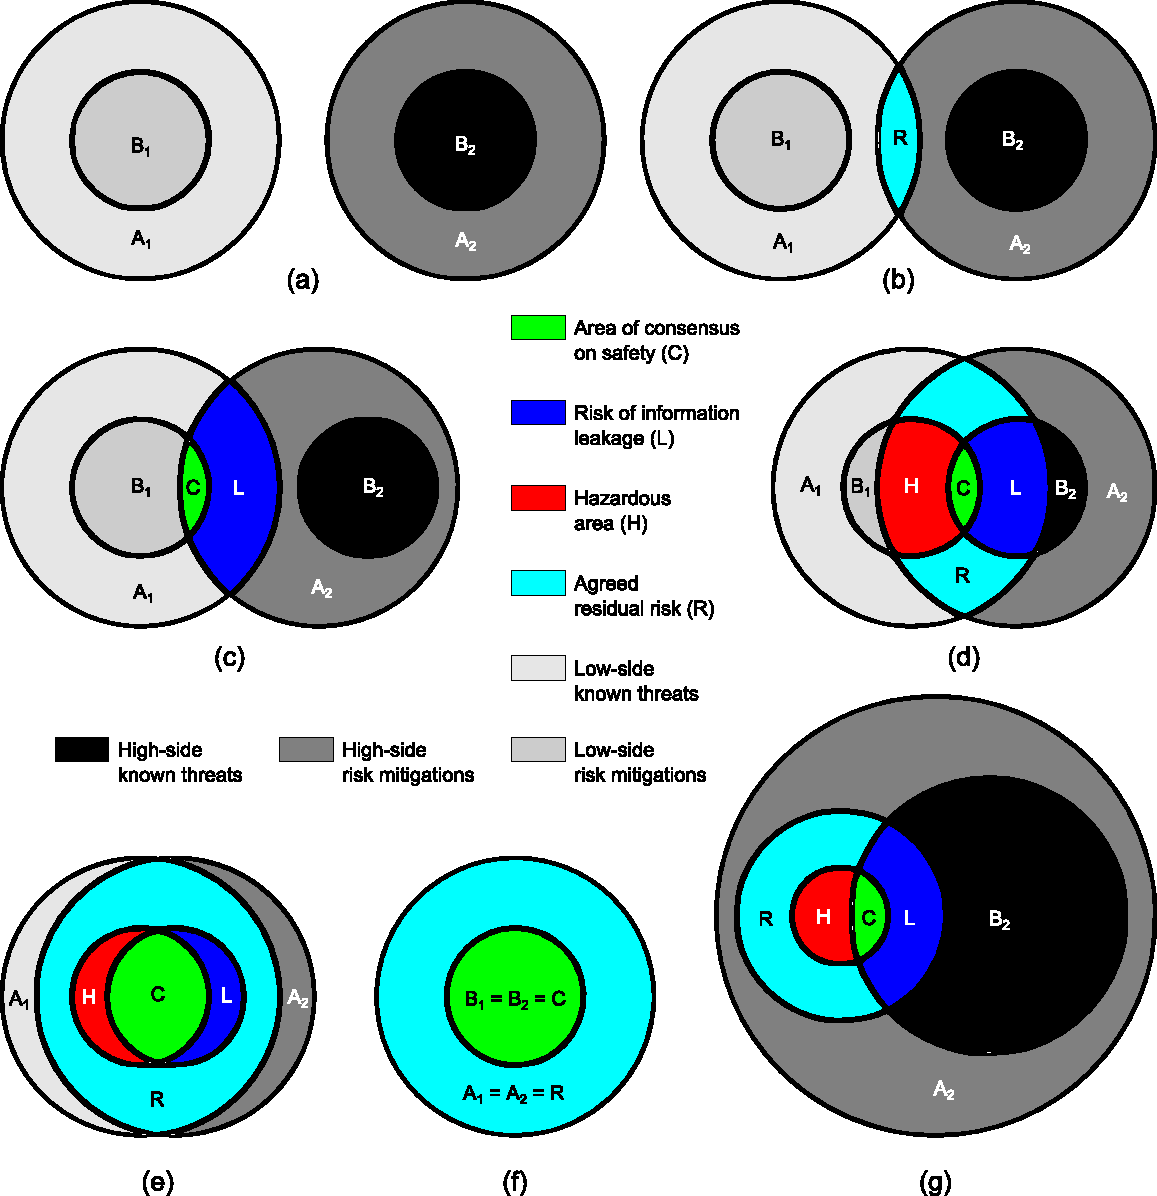
\includegraphics[width=\textwidth,trim=0 0 0 0, clip]{venn_diagrams_for_paper-corrected_without_fonts.pdf}
	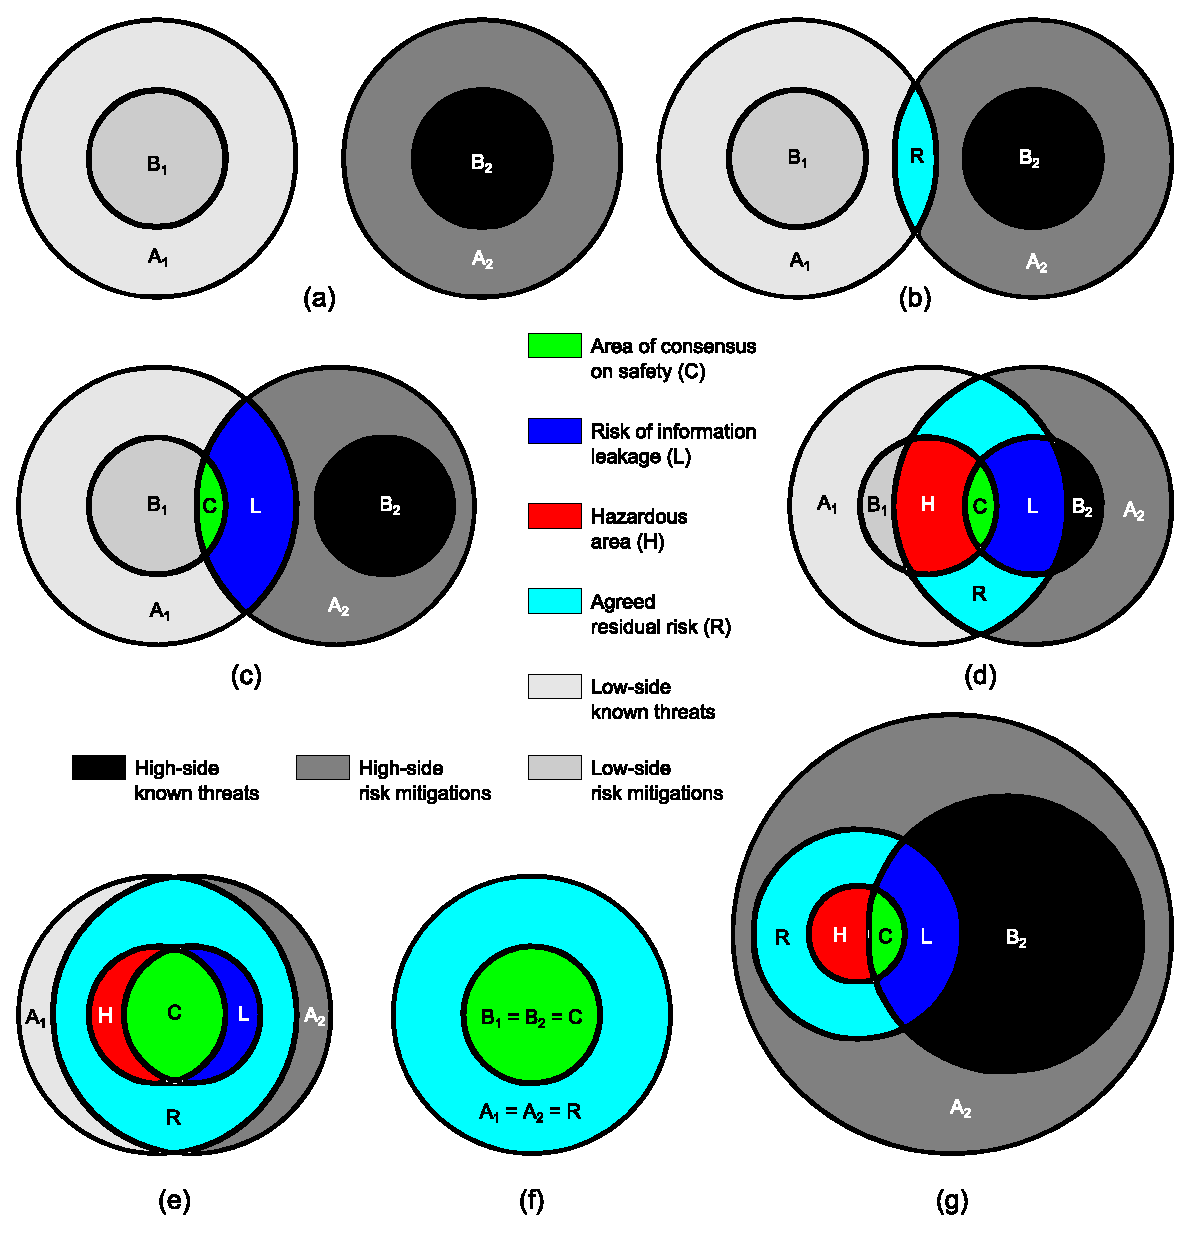
\includegraphics[width=\textwidth,bb=0 0 557 576]{venn_diagrams_for_paper-corrected.eps}
	\caption{In sub-figure (a), which represents a pure SCI-type international accreditation,
		Accreditor 1 has a completely independent idea of what threats exist ($A_1$) and what
		risk mitigations are possible ($A_2$); similarly, Accreditor 2 is cognisant of a
		different set of risks ($A_2$) that would be desirable to mitigate, and a smaller
		set ($B_2$) of risks that are, from Accreditor 2's perspective, possible to mitigate.
		Sub-figure (b) represents public information. Sub-figure (c) represents classified
		information with a risk of information leakage. In sub-figure (d) there is not only
		a risk of information leakage but personal risk to Accreditor 2 as well. Sub-figure
		(e) shows how the risk of classified information leakage and personal risk to one or
		more accreditors diminishes as the situation approaches a pure collateral configuration.
		Sub-figure (f) is the degenerate configuration of a null cross domain system.
		Sub-figure (g) shows a collateral (non-SCI-like) accreditation in which Accreditor 1
		has a lower security clearance than Accreditor 2; in this example, Accreditor 2 knows
		everything Accreditor 1 knows, but Accreditor 1 does not know everything Accreditor 2
		knows.}
		\label{figure:accreditor-model}
\end{figure*}

\subsection{Definitions}

Security classification levels for classified information may be hierarchical or non-hierarchical.
\emph{Collateral} classifications are hierarchical, ranging from unclassified through CONFIDENTIAL,
SECRET, and TOP SECRET, and are used by the military. A different type of classification, used by
the intelligence community, is Sensitive Compartmented Information (SCI). SCI compartments are
non-hierarchical and non-comparable, and the number of them is unlimited. Collateral and SCI are
often used in concert; for example, a person with a TOP SECRET clearance would have access to
CONFIDENTIAL information, but not SECRET CURVEBALL information, because CURVEBALL is (nominally)
SCI. However, a person with SECRET/SCI FASTBALL CURVEBALL KNUCKLEBALL clearance would have access,
assuming need-to-know.

\subsection{Cross Domain System Configurations}

Cross domain systems range in notional complexity from collateral, through mixed collateral-and-SCI,
to pure SCI-like systems, and finally those containing one or more international accreditors.
\figurename~\ref{figure:accreditor-model} shows the relationship amongst the types; they can best
be understood as a progression of overlapping knowledge. The larger circle, $A_i$, represents
the set of security controls that Accreditor $i$ thinks would be desirable to implement; this
corresponds to the threat as perceived by $i$. The smaller circle, $B_i$, represents the set of
security controls that Accreditor $i$ believes possible or affordable to implement. The area
between $A_i$ and $B_i$ is residual risk.

\subsubsection{Collateral Accreditations}

The simplest cross domain system is a collateral accreditation, meaning that all of the security
classifications are related hierarchically. This is the the Bell--LaPadula model \cite{Bell1973}.
As shown in \figurename~\ref{figure:accreditor-model}(g), because both
accreditors work for the same agency (e.g., the United States Department of Defence), it is often
the case that the high-side accreditor may be aware of all of the lower-classified security threats
and mitigations that the low-side accreditor is cleared to know about, but the high-side accreditor
additionally may know of other, more highly classified threats or risk mitigations that the
low-side accreditor is not cleared to know about. In the worst case, the high-side accreditor may
even have the guilty knowledge that certain risk mitigations trusted by the low-side accreditor are
ineffective in the face of highly classified threats. This leads to an information gradient from
high to low that can, in some instances, force the high-side accreditor to reveal classified
information to the low-side accreditor (coloured red in
\figurename~\ref{figure:accreditor-model}(g)) in violation of the high-side accreditor's oath
to protect classified information. In other instances, coloured blue in
\figurename~\ref{figure:accreditor-model}(g), the low-side accreditor may be able to deduce
certain information above the low-side accreditor's security clearance from the fact
that the high-side accreditor refuses to accept the residual risk of the cross domain system
accreditation without saying why; this leaks information.

\subsubsection{SCI Accreditations}

In an uncomplicated SCI accreditation with no shared compartments, shown in
\figurename~\ref{figure:accreditor-model}(a), there is no risk of information leakage; each
accreditor performs the risk assessment calculation independently. In
\figurename~\ref{figure:accreditor-model}(b) there is public information; both accreditors
agree that region $R$ is an acceptable risk. In \figurename~\ref{figure:accreditor-model}(c),
there is a risk of information leakage from Accreditor 1
to Accreditor 2, because Accreditor 1 considers region $C$ to pose an unacceptable risk, and by
insisting on the security controls in region $C$, inadvertently communicates to Accreditor 2 the
existence of a classified threat mitigation that Accreditor 2 is not cleared to know about.
\figurename~\ref{figure:accreditor-model}(d) is where it gets interesting. In configuration (d),
both accreditors may be aware of SCI threat mitigations that they are not allowed to tell the other
accreditor about, but in addition at least one accreditor may have guilty knowledge that some
threat mitigations (in region $H$) believed effective by the other accreditor do not
work.\footnote{Alternatively, it may be interpreted as knowledge of both the existence of
a classified threat and the fact that there is no known mitigation for it. When this situation
occurs in a collateral accreditation, there is no risk of information leakage because from the
perspective of the high-side accreditor, it is a risk he or she cannot talk about, and for the
low-side accreditor, ignorance is bliss.}

As the overlap grows between SCI accreditors, as in \figurename~\ref{figure:accreditor-model}(e),
the hazardous region $H$ shrinks, until the degenerate case of
\figurename~\ref{figure:accreditor-model}(f) where both sides of the cross domain system have
the same security clearance and classification.

\subsubsection{SCI-like and International Accreditations}

In the real world, things do not always seem so clear-cut. Cross domain systems interconnecting
international partners, or unclassified systems (such as news feeds) are not uncommon. It can
readily been seen, however, that the accreditor model accommodates such complications with ease, as
both international accreditors and unclassified endpoints can simply be treated as SCI
systems that happen to share no compartments. The model is therefore complete.

\section{Summary and Conclusion}

Cross domain systems, by definition, inhabit a niche where they necessarily always involve at
least two mutually distrustful data owners. Consequently, the security certification and
accreditation testing of components and systems will always tend to be rigorous. Previously it has
been shown that apparently unnecessary duplication of effort exists in the testing of cross domain
solutions and cross domain systems, but now it is beginning to be understood why this has occurred.
A grounded theory analysis of several variably successful case studies of cross domain
certification and accreditation projects led to the development of an abstract model of accreditor
behaviour suggesting that some disagreements, by reason of individual perspective from different
sides of a cross domain system, must lead to some amount of duplicated testing effort in order to
reach a consensus between accreditors with different---and sometimes incompatible---security
clearances.

\section{Acknowledgements}

Grateful acknowledgement is hereby given to the Lockheed Martin Corporation for access to
project records and data. The author wishes particularly to thank his supervisors, Dr Andrew
Martin and Dr Ivan Fl\'{e}chais for their insightful criticism of the accreditor model and
its applicability.

\section{Author Biography}

Joe Loughry received the B.A.\ degree in mathematics from the University of Colorado,
Boulder in 1986 and the M.S.E.\ degree in software engineering from Seattle University
in 1996; he is currently a Ph.D.\ student in computer science at the University of Oxford.
He did some of the first research on compromising optical
emanations and holds U.S.\ patent 6,987,461 on countermeasures. His research interests
include cross domain systems, certification and accreditation testing,
penetration testing, side channels, and efficient enumeration of subsets.

\bibliographystyle{IEEEtran}
\bibliography{IEEEabrv,consolidated_bibtex_file}

\end{document}

